\section{Theory}

\subsection{Begriffe und Klassifikation}

\subsubsection{Ordnung}

Wie bei gew�hnlichen Differentialgleichungen ist die Ordnung
die h�chste Ableitung der unbekannten Funktion, die in der
Differentialgleichung vorkommt.\\

\textbf{PDGL 1.Ordnung: } \qquad$F\biggl(x_1,\dots,x_n, u, \frac{\partial u}{\partial x_1},\dots,\frac{\partial u}{\partial x_n}\biggr)$

Sie kann durch Substitution $\frac{\partial u}{\partial x_i}\to p_i$ durch  $F(x_1,\dots,x_n,u,p_1,\dots,p_n),$
ausgedr�ckt werden.\\

\textbf{PDGL 2.Ordnung: } \qquad $F\biggl(x_1,\dots,x_n,u,
\frac{\partial u}{\partial x_1},\dots,\frac{\partial u}{\partial x_n},
\frac{\partial^2 u}{\partial x_1^2},\dots,\frac{\partial^2 u}{\partial x_n^2}\biggr)$

Sie kann durch Substitution $\frac{\partial u}{\partial x_i}\to p_i,~\frac{\partial^2 u}{\partial x_i\partial x_j}\to t_{ij}$ durch
$F(x_1,\dots,x_n,u,p_1,\dots,p_n,t_{11},t_{12},\dots,t_{n,n-1},t_{nn})$
ausgedr�ckt werden.

\subsubsection{Laplace-Operator}
$u(x,y,z)\quad\Rightarrow\quad \Delta u=\frac{\partial^2u}{\partial x^2}+\frac{\partial^2u}{\partial y^2}+\frac{\partial^2u}{\partial z^2}$

\subsubsection{Umwandlung in System niedriger Ordnung}

\begin{tabular}{ll}
Gegeben:& $F\biggl(x,y,u,\frac{\partial u}{\partial x},\frac{\partial u}{\partial y},
\frac{\partial^2 u}{\partial x^2},\frac{\partial^2 u}{\partial x\partial y},
\frac{\partial^2u}{\partial y^2}\biggr)=0.$\\[0.2cm]
Substitution: & $p=\frac{\partial u}{\partial x},\qquad q=\frac{\partial u}{\partial y}$\\[0.2cm]
F�r zweite Ableitungen: & $\frac{\partial^2 u}{\partial x^2}=\frac{\partial p}{\partial x},\quad \frac{\partial^2 u}{\partial x\partial y}=\frac{\partial p}{\partial y}=\frac{\partial q}{\partial x},\quad\frac{\partial^2 u}{\partial y^2}=\frac{\partial q}{\partial y}$\\[0.2cm]
Gleichungssystem 1.Ordnung& $p=\frac{\partial u}{\partial x},\quad q=\frac{\partial u}{\partial y},\quad\frac{\partial p}{\partial y}=\frac{\partial q}{\partial x}$
\end{tabular}

\subsubsection{Notationen einer PDGL, Gebiet $\Omega$}
\begin{minipage}{4cm}
	\begin{tabular}{ll}
	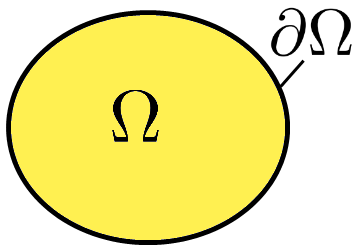
\includegraphics[width=3cm]{Content/Theory/Gebiet}&
	\end{tabular}
\end{minipage}
\begin{minipage}{4cm}	
	\begin{tabular}{ll}
		$\overset{\circ}{\Omega}$ & Innere Punkte\\
		$\partial\Omega$ & Rand\\
		$\overset{\_}{\Omega}$ & Gebiet $\Omega$ und Rand $\partial\Omega$\\
	\end{tabular}
\end{minipage}

Das Gebiet einer PDGL \textbf{muss} offen sein, nur dann ist die partielle Ableitung �berall definiert. Das Gebiet ist offen, wenn um jeden Punkt in Gebiet $\Omega$ ein kleiner Ball gezeichnet werden kann, welcher auch in Gebiet $\Omega$ ist.

\textbf{L�sung einer PDGL:}\\
\begin{tabular}{ll}
Gegeben:& Gebiet $\Omega$,PDGL,Randwerte $\partial\Omega$\\
L�sung:& Funktion $u$: $\overset{\_}{\Omega}\rightarrow \mathbb{R}$, PDGL in $\Omega$ und Randwerte auf $\partial\Omega$\\
\end{tabular}

\subsubsection{Klassifikation einer PRGL}


\begin{tabular}{ll}
Ordnung:& H�chste vorkommende partielle Ableitung\\
Type:& Linear:\qquad $F(\ldots)$ lineare Funktion von $u,\frac{\partial u}{\partial x_1},\frac{\partial u}{\partial x_2},\ldots,\frac{\partial u}{\partial x_n}$\\
& Quasilinear: \qquad  $F(\ldots)$ lineare Funktion von $u,\frac{\partial u}{\partial x_1},\frac{\partial u}{\partial x_2},u\frac{\partial u}{\partial x_k},\ldots,\frac{\partial u}{\partial x_n}$, wobei Produkte von \\

\todo{Anschauen}
\end{tabular}

\subsection{Charakteristiken}
\textbf{Wichtig:} Als Anfangsbedingungen dürfen \textbf{keine} Charakteristiken verwendet werden, sonst ist die Charakteristik die Lösung (anstatt Fläche ergibt sich eine Kurve).\\
\textbf{Wichtig:} Die Charakteristik darf den Rand nur einmal durchlaufen.\\
Nützlich für Qasilineare PDGL 1.Ordnung.\todo{Noch mehr?}\\
$$a(x,y,u)\cdot\partFrac{u}{x}+b(x,y,u)\cdot\partFrac{u}{y}=c(x,y,u) \qquad\Rightarrow\qquad a(x,y,u)\cdot\partFrac{u}{x}+b(x,y,u)\cdot\partFrac{u}{y}-c(x,y,u)=0$$\\


\begin{tabular}{ll}
Gebiet:& $\Omega{\ldots|x>0,alle y}$\qquad Randbedingung: $u(0,y_0)=g(y_0)$\\
Vektorielle schreibweise:& $\begin{bmatrix}
	a(x,y,u)\\ b(x,y,u)\\ c(x,y,u)
\end{bmatrix}\cdot 
\underset{\overrightarrow{n}~:~Normale ~auf~ Flaeche}{\underbrace{\begin{bmatrix}
\partFrac{u}{x} & \partFrac{u}{y} & -1
\end{bmatrix}}}=0$\\[1cm]
Tangenten:& $\overrightarrow{t}_x=\begin{bmatrix}1\\0\\ \partFrac{u}{x}\end{bmatrix}\qquad 
			\overrightarrow{t}_y=\begin{bmatrix}0\\1\\ \partFrac{u}{y}\end{bmatrix}$\\[1cm]
Lösungsweg& Für jeden Anfangspunkt $\begin{bmatrix} 0\\y_0\\g(y_0)\end{bmatrix}$ finde eine Charakteristik, diese nach $x$, $y$ auflösen.
\end{tabular}

Beispiel:\\
\begin{enumerate}
	\item PDGL mit Randbedingungen und Definitionsbereich: $\partFrac ux+2\partFrac uy=3$, \; $u(0,y)=g(y)=\sin(y) \Rightarrow u(0,y_0) = g(y_0) = \sin(y_0)$\\
	Therme in Matrixschreibweise: $\begin{bmatrix}a\\b\\c\end{bmatrix}=\begin{bmatrix}1\\2\\3\end{bmatrix}$
	\item Charakteristiken ausrechnen PDGL $\rightarrow$ DGL: 	$\frac {d}{dt}\begin{bmatrix}x(t)\\y(t)\\u(t)\end{bmatrix}=\begin{bmatrix}1\\2\\3\end{bmatrix}$
	\item DGL's lösen (für Standard-DGLS, siehe \ref{sec:dgls} auf Seite \pageref{sec:dgls}.): 
	$\begin{bmatrix}x\\y\\u\end{bmatrix}=\begin{bmatrix}t+x_0\\t+y_0\\t+u_0\end{bmatrix}$
	\item Anfangsbedingungen einsetzen: $\begin{bmatrix}x\\y\\u\end{bmatrix}=\begin{bmatrix}t+x_0\\t+y_0\\t+u_0\end{bmatrix}\Bigg|_{t=0}=
	\begin{bmatrix}x_0\\y_0\\u_0\end{bmatrix}=\begin{bmatrix}0\\y_0\\\sin(y_0)\end{bmatrix}$\\
	Lösung der DGL ist: $\begin{bmatrix}x\\y\\u\end{bmatrix}=\begin{bmatrix}1\\2\\3\end{bmatrix}\cdot t+ \begin{bmatrix}0\\y_0\\\sin(y_0)\end{bmatrix}$\\
	
	\item Eliminieren aller Variablen ausser $u,x,y$: $u=3x+\sin(y-2x)$
	\item Kontrolle
	Resultat ($u=3x+\sin(y-2x)$) ableiten und in Aufgabenstellung einsetzen $\partFrac ux+2\partFrac uy=3$ und schauen ob es erfüllt.
	
\end{enumerate}



\subsection{Methode Separation}
Wahl eines geeigneten Koordinatensystems ist wichtig.


\begin{enumerate}
\item \textbf{Ansatz} (Höchste Ableitung ausschlaggebend): 
	\begin{itemize}
		\item Für PDGL 1.Ordnung: $U(x,y)=X(x) + Y(y)$
		\item Für PDGL 2.Ordnung: $U(x,y)=X(x) \cdot Y(y)$ 
	\end{itemize}
\item \textbf{Einsetzen: } Ansatz in PDGL einsetzen.
\item \textbf{Separation: } Auf jeder Seite der PDGL darf nur noch eine Variable vorkommen. Die beiden jetzt gewöhnlichen DGL sind über eine Konstante gekoppelt (fixieren der Variable). Wahl der Konstante: Wenn Schwingung erwartet wird: $-k^2$, sonst $k$, ausser man weiss es besser ;-).
\item \textbf{Lösen der DGL's: } Man erhält eine Familie von Lösungen	
\item \textbf{Gesamtlösung "'Zusammenbasteln"': } (Linearkombination der Lösungen), Randbedingungen einhalten!
\end{enumerate}

\begin{minipage}{0.49\textwidth}
\textbf{Beispiel 1: } PDGL: $\frac1x\partFrac{u}{x}+\frac1y\partFrac{u}{y}=\frac{1}{y^2}$
\begin{enumerate}
	\item Ansatz:\\[0.4cm]
	$u(x,y)=X(x) + Y(y)$ (1.Ordnung)
	\item Einsetzen:\\[0.4cm]
	$\partFrac{u}{x}=X'(x)$\qquad $\partFrac{u}{y}=Y'(y)$ \quad $\Rightarrow$ \quad $\frac{X'(x)}{x}+\frac{Y'(y)}{y}=\frac{1}{y^2}$
	\item Separation:\\[0.4cm]
	$\frac{X'(x)}{x}=k=\frac{1}{y^2}-\frac{Y'(y)}{y}$
	\item DGL'2 lösen:\\[0.4cm]
	$X'(x)=k\cdot x \quad\Rightarrow\quad X(x)=\frac12 kx^2+C_x$\\
	$Y'(y)=\frac1y-ky \quad\Rightarrow\quad Y(y)=\ln(y)-\frac12 ky^2+C_y$
	\item Linearkombination:\\[0.4cm]
	$u(x,y)=\frac12 kx^2 - \frac12 ky^2+ln(y)+C$
\end{enumerate}

\textbf{Beispiel 2: } PDGL: $x^2\partFrac{^2u}{x^2}+x\partFrac{u}{x}+y^2\partFrac{^2u}{y^2}+y\partFrac{u}{y}=0$\\ 
Randbedingungen: $\Omega=[1,2]\times[1,2]$ \qquad $u=0$ auf $\partial\Omega$
\begin{enumerate}
	\item Ansatz:\\[0.4cm]
	$u(x,y)=X(x) \cdot Y(y)$ (2.Ordnung)
	\item Einsetzen:\\[0.4cm]
	$x^2X''(x)Y(y)+xX'(x)Y(y)+y^2X(x)Y''(y)+yX(x)Y'(y)=0$
	\item Separation: Division durch $X(x)Y(y)$\\[0.4cm]
	$\frac{x^2X''(x)}{X(x)}+\frac{xX'(x)}{X(x)}+\frac{y^2Y''(y)}{Y(y)}+\frac{yY'(y)}{Y(y)}=0\quad\Rightarrow\quad \frac{x^2X''(x)}{X(x)}+\frac{xX'(x)}{X(x)}=k=-\frac{y^2Y''(y)}{Y(y)}-\frac{yY'(y)}{Y(y)}$
	\item DGL'2 lösen:\\[0.4cm]
	$\frac{x^2X''(x)}{X(x)}+\frac{xX'(x)}{X(x)}=k\quad\Rightarrow\quad x^2X''(x)+xX'(x)-kX(x)=0$\qquad mit $X(1)=X(2)=0$\\
	$\frac{y^2Y''(y)}{Y(y)}-\frac{yY'(y)}{Y(y)}=-k\quad\Rightarrow\quad y^2Y''(y)+yY'(y)+kY(y)=0$\qquad mit $Y(1)=Y(2)=0$\\[0.4cm]
	Lösung der DGL hier nicht gemacht.
\end{enumerate}
\end{minipage}
\hfill
\begin{minipage}{0.49\textwidth}
\textbf{Beispiel 3: }PDGL: $\partFrac{^2u}{t^2}=\partFrac{^2u}{x^2}$ \quad $u(t=0,x)=0$\\
Randbedingungen: $x=[0,\pi]$ \\
\qquad\qquad $\partFrac{u}{t}(t=0,x)=\sin^3(x)=\frac34\sin(x)-\frac14\sin(3x)$
\begin{enumerate}
	\item Ansatz:\\[0.4cm]
	$u(t,x)=T(t) \cdot X(x) $ (2.Ordnung)
	\item Einsetzen:\\[0.4cm]
	$T''(t)\cdot X(x) = X''(x)\cdot T(t)$
	\item Separation:\\[0.4cm]
	$\frac{X''(x)}{X(x)}= -\mu^2=\frac{T''(t)}{T(t)}$
	\item DGL'2 lösen:\\[0.4cm]
		$X(x)=\sin(\mu x) \qquad T(t)=\sin(\mu t)$\\
		$X(x)=\cos(\mu x) \qquad T(t)=\cos(\mu t)$
	\item Linearkombination:\\[0.4cm]
		Die Randbedingungen $x=0$ und $x=\pi$ können nur mit $\sin(\mu x) $ und  positivem, ganzzahligen $\mu$ erfüllt werden. $cos(nx)$-Therme fallen weg.\\[0.4cm]
		$u(t,x)=\sum\limits_{n=1}^{\infty}{a_n\sin(nx)\sin(nt)} + \sum\limits_{n=1}^{\infty}{b_n\sin(nx)\cos(nt)}$\\[0.4cm]
		Die Koeffizienten $a_n$ und $b_n$ müssen mit Hilfe der Anfangsbedingungen zur Zeit $t=0$ bestimmt werden:\\[0.4cm]
		$u(0,x)=\sum\limits_{n=1}^{\infty}{b_n\sin(nx)}=0 \quad\Rightarrow\quad b_n=0$\\[0.2cm]
		$\partFrac{u}{t}(\pi,x)=\sum\limits_{n=1}^{\infty}{a_nn\sin(nx)}=\sin^3(x)=\frac34\sin(x)-\frac14\sin(3x) \quad\Rightarrow\quad a_1=\frac34 \quad a_3=-\frac{1}{12}\quad a_k=0$ für $k\neq 1,3$\\[0.4cm]
		$u(t,x)=\frac34\sin(x)\sin(t)-\frac1{12}\sin(3x)\sin(3t)$
\end{enumerate}
\end{minipage}









